\documentclass[14pt]{extbook}
\usepackage{multicol, enumerate, enumitem, hyperref, color, soul, setspace, parskip, fancyhdr} %General Packages
\usepackage{amssymb, amsthm, amsmath, bbm, latexsym, units, mathtools} %Math Packages
\everymath{\displaystyle} %All math in Display Style
% Packages with additional options
\usepackage[headsep=0.5cm,headheight=12pt, left=1 in,right= 1 in,top= 1 in,bottom= 1 in]{geometry}
\usepackage[usenames,dvipsnames]{xcolor}
\usepackage{dashrule}  % Package to use the command below to create lines between items
\newcommand{\litem}[1]{\item#1\hspace*{-1cm}\rule{\textwidth}{0.4pt}}
\pagestyle{fancy}
\lhead{Progress Quiz 3}
\chead{}
\rhead{Version A}
\lfoot{}
\cfoot{}
\rfoot{Fall 2020}
\begin{document}

\begin{enumerate}
\litem{
Solve the radical equation below. Then, choose the interval(s) that the solution(s) belongs to.\[ \sqrt{-49 x^2 + 15} - \sqrt{-14 x} = 0 \]\begin{enumerate}[label=\Alph*.]
\item \( \text{All solutions lead to invalid or complex values in the equation.} \)
\item \( x_1 \in [-0.27, 0.45] \text{ and } x_2 \in [-1.29,1.71] \)
\item \( x_1 \in [-1.17, -0.03] \text{ and } x_2 \in [-1.29,1.71] \)
\item \( x \in [0.67,1.33] \)
\item \( x \in [-1.17,-0.03] \)

\end{enumerate} }
\litem{
Solve the radical equation below. Then, choose the interval(s) that the solution(s) belongs to.\[ \sqrt{-7 x - 5} - \sqrt{5 x + 2} = 0 \]\begin{enumerate}[label=\Alph*.]
\item \( \text{All solutions lead to invalid or complex values in the equation.} \)
\item \( x_1 \in [-0.85, -0.66] \text{ and } x_2 \in [-1.01,-0.46] \)
\item \( x \in [-0.45,-0.18] \)
\item \( x_1 \in [-0.85, -0.66] \text{ and } x_2 \in [-0.41,1.37] \)
\item \( x \in [-0.68,-0.27] \)

\end{enumerate} }
\litem{
Choose the equation of the function graphed below.
\begin{center}
    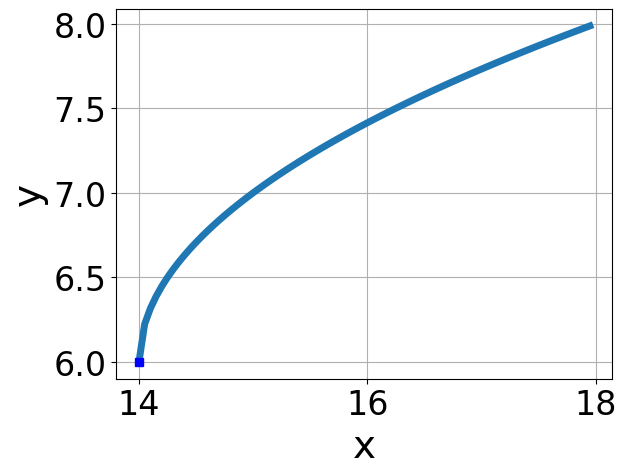
\includegraphics[width=0.5\textwidth]{../Figures/radicalGraphToEquationA.png}
\end{center}
\begin{enumerate}[label=\Alph*.]
\item \( f(x) = - \sqrt{x - 8} + 4 \)
\item \( f(x) = - \sqrt{x + 8} + 4 \)
\item \( f(x) = \sqrt{x - 8} + 4 \)
\item \( f(x) = \sqrt{x + 8} + 4 \)
\item \( \text{None of the above} \)

\end{enumerate} }
\litem{
Solve the radical equation below. Then, choose the interval(s) that the solution(s) belongs to.\[ \sqrt{-21 x^2 - 42} - \sqrt{-67 x} = 0 \]\begin{enumerate}[label=\Alph*.]
\item \( x \in [2.06,2.43] \)
\item \( \text{All solutions lead to invalid or complex values in the equation.} \)
\item \( x \in [0.6,1.44] \)
\item \( x_1 \in [0.6, 1.44] \text{ and } x_2 \in [2.33,3.33] \)
\item \( x_1 \in [-1.01, -0.35] \text{ and } x_2 \in [-4.33,1.67] \)

\end{enumerate} }
\litem{
Choose the equation of the function graphed below.
\begin{center}
    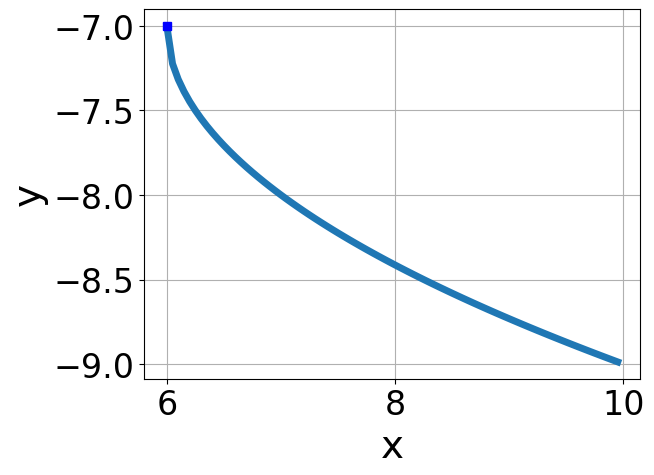
\includegraphics[width=0.5\textwidth]{../Figures/radicalGraphToEquationCopyA.png}
\end{center}
\begin{enumerate}[label=\Alph*.]
\item \( f(x) = - \sqrt{x + 14} - 3 \)
\item \( f(x) = \sqrt{x - 14} - 3 \)
\item \( f(x) = - \sqrt{x - 14} - 3 \)
\item \( f(x) = \sqrt{x + 14} - 3 \)
\item \( \text{None of the above} \)

\end{enumerate} }
\litem{
Choose the graph of the equation below.\[ f(x) = \sqrt[3]{x + 6} + 7 \]\begin{enumerate}[label=\Alph*.]
\begin{multicols}{2}\item 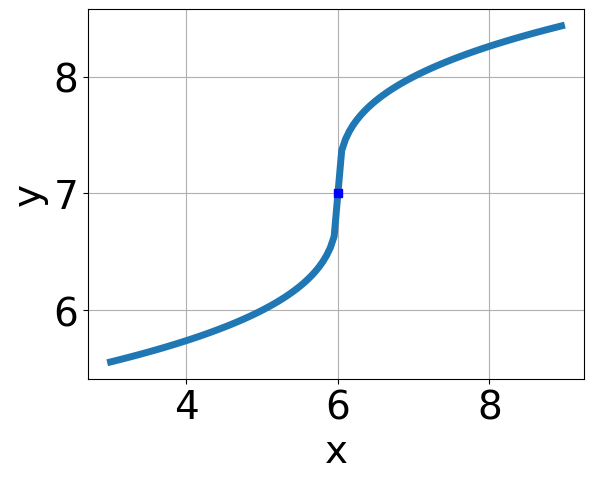
\includegraphics[width = 0.3\textwidth]{../Figures/radicalEquationToGraphCopyAA.png}\item 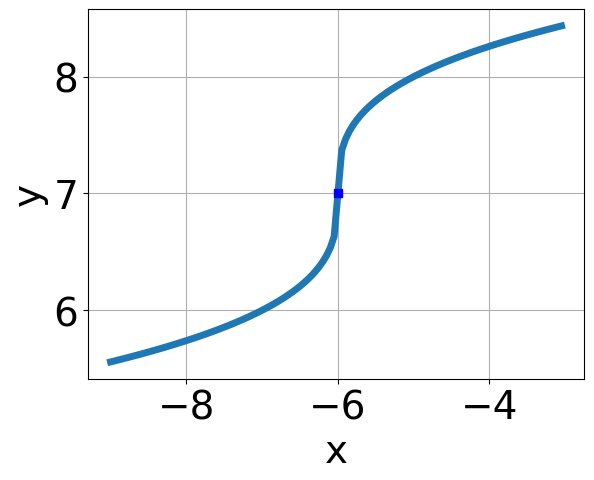
\includegraphics[width = 0.3\textwidth]{../Figures/radicalEquationToGraphCopyBA.png}\item 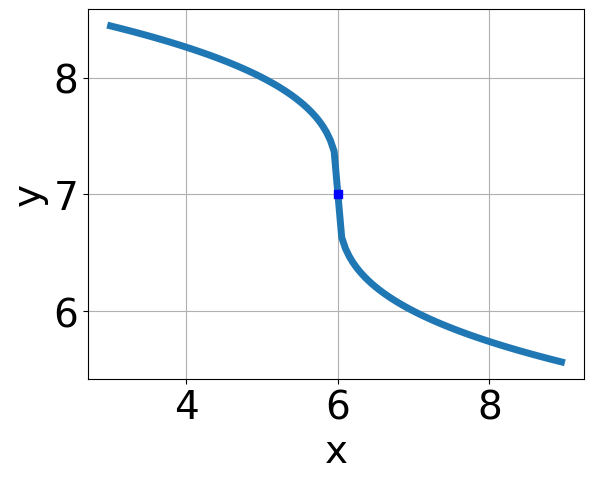
\includegraphics[width = 0.3\textwidth]{../Figures/radicalEquationToGraphCopyCA.png}\item 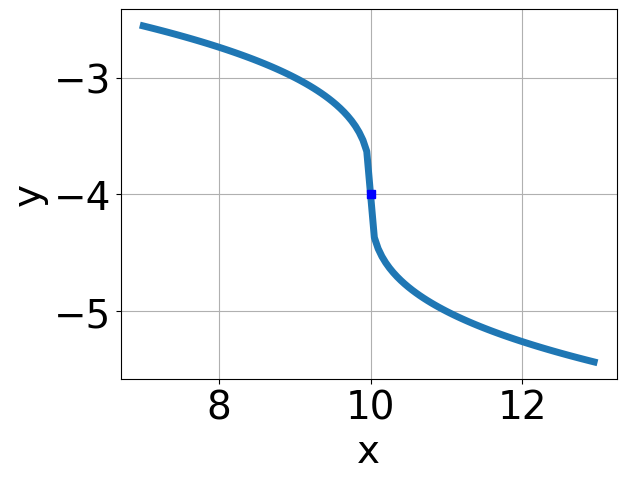
\includegraphics[width = 0.3\textwidth]{../Figures/radicalEquationToGraphCopyDA.png}\end{multicols}\item None of the above.
\end{enumerate} }
\litem{
What is the domain of the function below?\[ f(x) = \sqrt[3]{4 x - 8} \]\begin{enumerate}[label=\Alph*.]
\item \( \text{The domain is } [a, \infty), \text{   where } a \in [-1.8, 1.3] \)
\item \( \text{The domain is } (-\infty, a], \text{   where } a \in [0.22, 1.96] \)
\item \( \text{The domain is } [a, \infty), \text{   where } a \in [0.6, 2.5] \)
\item \( (-\infty, \infty) \)
\item \( \text{The domain is } (-\infty, a], \text{   where } a \in [0.84, 2.71] \)

\end{enumerate} }
\litem{
Choose the graph of the equation below.\[ f(x) = - \sqrt[3]{x - 8} + 6 \]\begin{enumerate}[label=\Alph*.]
\begin{multicols}{2}\item 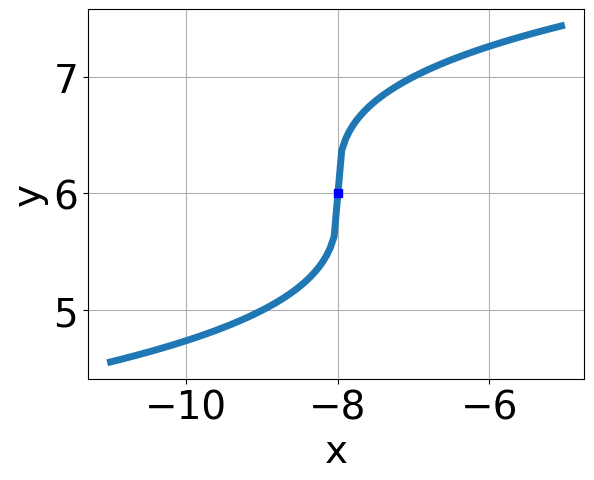
\includegraphics[width = 0.3\textwidth]{../Figures/radicalEquationToGraphAA.png}\item 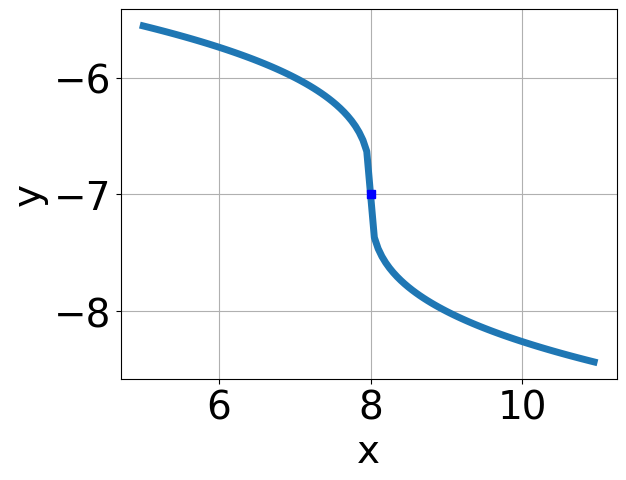
\includegraphics[width = 0.3\textwidth]{../Figures/radicalEquationToGraphBA.png}\item 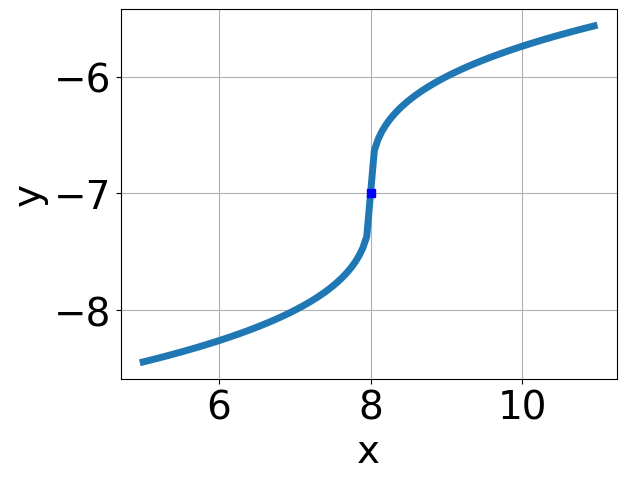
\includegraphics[width = 0.3\textwidth]{../Figures/radicalEquationToGraphCA.png}\item 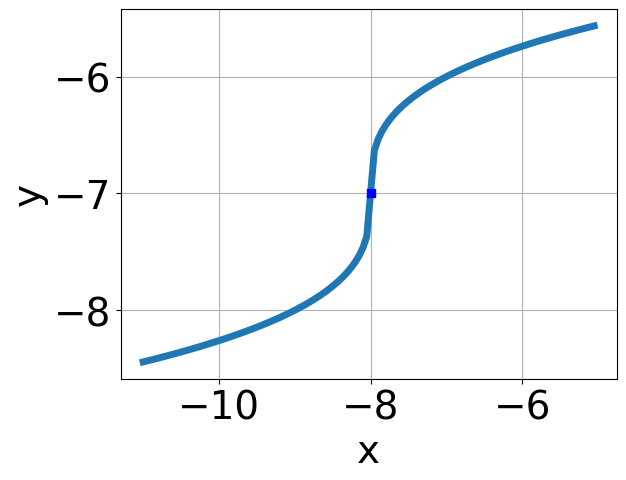
\includegraphics[width = 0.3\textwidth]{../Figures/radicalEquationToGraphDA.png}\end{multicols}\item None of the above.
\end{enumerate} }
\litem{
Solve the radical equation below. Then, choose the interval(s) that the solution(s) belongs to.\[ \sqrt{9 x - 7} - \sqrt{4 x + 2} = 0 \]\begin{enumerate}[label=\Alph*.]
\item \( \text{All solutions lead to invalid or complex values in the equation.} \)
\item \( x_1 \in [0.75, 0.84] \text{ and } x_2 \in [1.5,2.5] \)
\item \( x_1 \in [-0.71, -0.38] \text{ and } x_2 \in [-0.6,1.6] \)
\item \( x \in [1,1.13] \)
\item \( x \in [1.77,1.87] \)

\end{enumerate} }
\litem{
What is the domain of the function below?\[ f(x) = \sqrt[3]{-4 x + 6} \]\begin{enumerate}[label=\Alph*.]
\item \( \text{The domain is } (-\infty, a], \text{   where } a \in [1.22, 2.13] \)
\item \( \text{The domain is } [a, \infty), \text{   where } a \in [0.99, 2.22] \)
\item \( (-\infty, \infty) \)
\item \( \text{The domain is } (-\infty, a], \text{   where } a \in [0.58, 1.23] \)
\item \( \text{The domain is } [a, \infty), \text{   where } a \in [0.56, 1.14] \)

\end{enumerate} }
\end{enumerate}

\end{document}